\section{相对密度}
\label{sec:density-relative}

本节固定同一可测空间$(X,\mathcal A)$上的两个非负测度：一个充当参考，一个是要描述的目标。先在有限点集上看清“密度就是质量之比”，再借助第~\ref{chap:integration}章的积分把这个想法推广到一般测度。随后从相反的方向说明：任给参考测度和非负权重，积分总能产生一个新测度；最后说明密度只在参考测度的几乎处处意义下有意义。

\subsection{参考测度与密度的定义}
\label{sec:density-definition}

\paragraph{有限点集上的质量之比}
设$X=\{a,b,c\}$，目标测度$\nu$给三个点的质量分别为$0.2,0.5,0.3$。若参考测度是计数测度，每点质量为$1$，那么要从参考质量得到目标质量，只需在每点乘以$0.2,0.5,0.3$。若参考测度改为$\mu'=2\delta_a+\delta_b+\delta_c$，点$a$的参考质量是$2$，乘数就要改成$0.2/2=0.1$，另外两点的乘数不变。一般地，参考测度在点$x_i$上的质量为$m_i>0$、目标质量为$p_i$时，该点的乘数是$p_i/m_i$；任一子集的目标质量都等于参考质量乘以乘数后求和，例如$\nu(\{a,b\})=0.1\cdot2+0.5\cdot1=0.7$。

图~\ref{fig:density-mass-ratio}并排画出这两种参考。读者应注意，目标测度在两栏中完全相同，变化的只有虚线框表示的参考质量，因而乘数$h$随之改变。密度描述的是“目标相对于参考”的换算比例，离开参考测度谈密度没有意义。

\begin{figure}[!htbp]
  \centering
  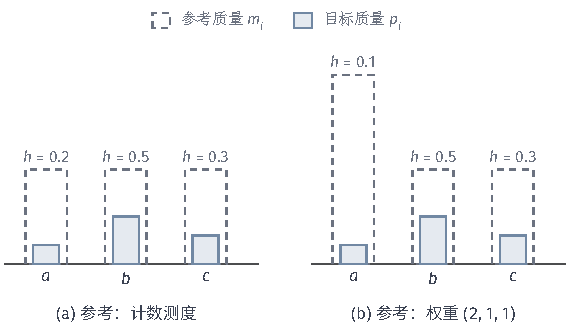
\includegraphics[width=96.651mm]{figures/02-abstract-mathematics/01-metric-and-measure/tikz/c4-mass-ratio/figure.pdf}
  \caption{密度是目标质量与参考质量之比。三点集$\{a,b,c\}$上的目标质量$p=(0.2,0.5,0.3)$（蓝色实心柱）保持不变。(a)参考为计数测度（虚线框高为$1$），每点的密度$h$等于目标质量本身；(b)参考权重改为$(2,1,1)$，点$a$的密度变为$0.2/2=0.1$，其余两点不变。}
  \label{fig:density-mass-ratio}
\end{figure}

\paragraph{一般测度上的密度}
有限点集上可以逐点做除法，是因为每一点都有正的参考质量。在实轴的长度测度下，每个单点的长度都是$0$，“单点质量相除”就成了$0/0$，所以一般情形不能逐点定义比值。可以保留的是另一半：在每个集合上，参考质量乘以权重再累计，应当得到目标质量。在有限点集上这个累计是求和，一般情形下就是第~\ref{chap:integration}章的积分。约定$\int_Ah\,\mathrm d\mu=\int_Xh\mathbf 1_A\,\mathrm d\mu$。

\begin{definition}[相对密度]
\label{def:density-density}
设$\mu,\nu$是可测空间$(X,\mathcal A)$上的非负测度。若可测函数$h:X\to[0,+\infty]$满足
\begin{equation}
 \nu(A)=\int_Ah\,\mathrm d\mu,\qquad A\in\mathcal A,
 \label{eq:density-definition}
\end{equation}
就称$h$是$\nu$相对于$\mu$的一个\term{相对密度}（relative density），也称\term{Radon–Nikodym密度}（Radon-Nikodym derivative），记作$\dfrac{\mathrm d\nu}{\mathrm d\mu}=h$；$\mu$称为\term{参考测度}（reference measure）。
\end{definition}

定义中说的是“一个”密度：后面会看到，在参考零测集上改动$h$不影响\eqref{eq:density-definition}，所以记号$\mathrm d\nu/\mathrm d\mu$只指其中任一个版本，含有它的等式都理解为$\mu$-几乎处处成立。这里没有新的积分理论，新增的只是用一个函数来表示两个测度之间的关系。记号$\mathrm d\nu/\mathrm d\mu$借用了导数的写法，但它不是对某个坐标求导，而是两种测度之间的换算权重。

\paragraph{概率质量函数与概率密度函数}
卷一用概率质量函数和概率密度函数描述随机变量的分布（可参考\BookChapterRef{chap:random-variables}{卷一“随机变量与概率分布”章}），二者都是上述定义的特例，区别只在参考测度。离散分布在可数集合$S$上的概率质量函数$p(s)$满足$\nu(A)=\sum_{s\in A}p(s)$；对计数测度$c$的积分就是求和（第~\ref{sec:integral-classical}节），所以$p$是$\nu$相对于$c$的密度。连续分布的概率密度函数$p$满足$\nu(A)=\int_Ap\,\mathrm d\lambda$，它是相对于Lebesgue测度$\lambda$的密度。

一般的密度不要求总积分为一：$\int_Xh\,\mathrm d\mu=\nu(X)$，只有目标测度是概率测度时这个值才是$1$。例如$[0,1]$上的$h(x)=2$是测度$2\lambda|_{[0,1]}$相对于$\lambda$的密度，总质量为$2$。另一方面，概率密度函数在某点的值可以大于$1$，因为它不是该点的概率；在长度测度下单点的概率总是$0$，密度值只有在集合上积分后才变成质量。

\subsection{由密度构造测度}
\label{sec:density-weighted-measure}

定义~\ref{def:density-density}是从两个已知测度出发的。反过来，若只给定参考测度和一个非负权重，按\eqref{eq:density-definition}的右边计算，是否总得到一个测度？答案是肯定的，而且不需要任何有限性条件。

\begin{theorem}[加权测度]
\label{thm:density-weighted-measure}
设$(X,\mathcal A,\mu)$是测度空间，$h:X\to[0,+\infty]$可测。令
\[
 \nu_h(A)=\int_Ah\,\mathrm d\mu,\qquad A\in\mathcal A .
\]
则$\nu_h$是$(X,\mathcal A)$上的非负测度，$h$是它相对于$\mu$的密度，并且$\nu_h\ll\mu$。
\end{theorem}

\begin{proof}
$\nu_h(\varnothing)=\int_X0\,\mathrm d\mu=0$，且$\nu_h$取值于$[0,+\infty]$。设$A_1,A_2,\dots\in\mathcal A$两两不交，$A=\bigcup_nA_n$。由于各$A_n$不交，$h\mathbf 1_A=\sum_{n=1}^\infty h\mathbf 1_{A_n}$逐点成立。部分和$g_N=\sum_{n=1}^Nh\mathbf 1_{A_n}$是非负可测函数，关于$N$单调递增并逐点收敛到$h\mathbf 1_A$。由非负积分的有限可加性，$\int_Xg_N\,\mathrm d\mu=\sum_{n=1}^N\nu_h(A_n)$；再由单调收敛定理（定理~\ref{thm:integral-monotone-convergence}），
\[
 \nu_h(A)=\int_Xh\mathbf 1_A\,\mathrm d\mu=\lim_{N\to\infty}\int_Xg_N\,\mathrm d\mu=\sum_{n=1}^\infty\nu_h(A_n).
\]
所以$\nu_h$可数可加，是测度。$h$满足\eqref{eq:density-definition}正是$\nu_h$的定义。若$\mu(A)=0$，函数$h\mathbf 1_A$在$\mu$零测集之外为零，其积分为$0$（第~\ref{sec:integral-properties}节），故$\nu_h(A)=0$，即$\nu_h\ll\mu$（定义~\ref{def:measure-absolutely-continuous}）。
\end{proof}

证明只用了积分的有限可加性和单调收敛，没有要求$\mu$或$h$有限。若$h$在一个正测度集合上取$+\infty$，$\nu_h$可能连$\sigma$有限都不是；它仍然是一个测度。定理的最后一句把加权构造与第~\ref{sec:measure-relations}节的绝对连续联系起来：凡是有密度的测度都相对于参考测度绝对连续。

\paragraph{分块加权}
当$h$是非负简单函数$h=\sum_{i=1}^mc_i\mathbf 1_{A_i}$，其中$A_1,\dots,A_m$两两不交且并为$X$，$c_i\in[0,+\infty)$，构造就回到分块乘系数。由简单函数积分的定义，
\[
 \nu_h(E)=\int_X\sum_{i=1}^mc_i\mathbf 1_{A_i\cap E}\,\mathrm d\mu=\sum_{i=1}^mc_i\,\mu(E\cap A_i),
\]
即在每一块上把参考质量乘以该块的系数再相加，这正是有限点集上逐点相乘的推广。在$[0,1]$上取$\mu=\lambda|_{[0,1]}$与
\[
 h=\tfrac32\mathbf 1_{[0,1/2)}+\tfrac12\mathbf 1_{[1/2,1]},
\]
则$\nu_h([0,1])=\tfrac32\cdot\tfrac12+\tfrac12\cdot\tfrac12=1$，$\nu_h$是概率测度；对$E=[1/4,3/4]$，$\nu_h(E)=\tfrac32\cdot\tfrac14+\tfrac12\cdot\tfrac14=\tfrac12$。图~\ref{fig:density-weighted-measure}(a)中这个值就是$E$上方、密度图像之下的阴影面积，左右两块分别贡献$3/8$与$1/8$。

\paragraph{两个方向}
到这里应当区分两个方向。“给定权重，产生测度”已经由定理~\ref{thm:density-weighted-measure}完全解决，对任何非负可测$h$都可行。“给定两个测度，寻找权重”则要问：是否存在同一个函数$h$，使\eqref{eq:density-definition}对所有可测集同时成立？由定理~\ref{thm:density-weighted-measure}，$\nu\ll\mu$是一个必要条件；它是否充分，以及需要什么附加条件，是第~\ref{sec:density-existence}节的内容。

\subsection{密度的几乎处处版本}
\label{sec:density-ae-version}

\paragraph{改动零测集不改变测度}
若可测函数$h,g\ge0$满足$h=g$ $\mu$-几乎处处，则对每个可测集$A$，$h\mathbf 1_A$与$g\mathbf 1_A$也$\mu$-几乎处处相等；几乎处处相等的非负可测函数积分相同（第~\ref{sec:integral-properties}节），所以$\nu_h(A)=\nu_g(A)$。换言之，密度在$\mu$零测集上的取值完全不能由集合质量确定。在$[0,1]$上，$h=1$与$g=1+\mathbf 1_{\mathbb Q\cap[0,1]}$都给出长度测度$\lambda|_{[0,1]}$，因为$g$只在可数集$\mathbb Q\cap[0,1]$上与$h$不同，而可数集是$\lambda$零测集。图~\ref{fig:density-weighted-measure}(b)画出了这种改动：红点处的函数值变了，阴影面积不变。

\begin{figure}[!htbp]
  \centering
  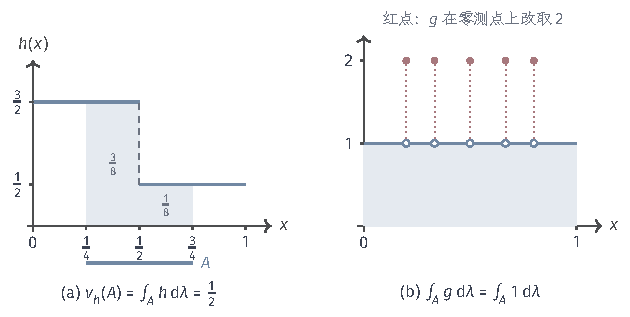
\includegraphics[width=106.684mm]{figures/02-abstract-mathematics/01-metric-and-measure/tikz/c4-weighted-measure/figure.pdf}
  \caption{由密度构造测度，以及几乎处处版本。(a)参考测度为$[0,1]$上的长度，密度$h$在$[0,1/2)$上取$3/2$、在$[1/2,1]$上取$1/2$；集合$A=[1/4,3/4]$的质量$\nu_h(A)$是$A$上方的阴影面积$3/8+1/8=1/2$。(b)常数密度$1$与在若干零测点（示意有理点）上改取$2$的函数$g$给出同一测度，因为改动的位置不承载长度。}
  \label{fig:density-weighted-measure}
\end{figure}

因此，说“$h$是$\nu$相对于$\mu$的密度”时，应当把与$h$几乎处处相等的所有函数看作同一个对象的不同版本；关于密度的逐点断言，如“$h>0$”“$h<\infty$”，都只在$\mu$-几乎处处的意义下才有意义。

\paragraph{正向结论与唯一性}
上面证明的是正向结论：几乎处处相等的函数产生同一个测度。密度的唯一性是反向的命题：若$h$与$g$产生同一个测度，能否推出它们几乎处处相等？这需要额外的有限性条件。取单点空间$X=\{0\}$，$\mu(\{0\})=+\infty$，$\nu=\mu$。常数$1$与常数$2$都满足$\int_{\{0\}}h\,\mathrm d\mu=+\infty=\nu(\{0\})$，可它们在一个$\mu$测度为$+\infty$的集合上不同。这里$\mu$不是$\sigma$有限的。第~\ref{sec:density-existence}节将在$\sigma$有限的条件下证明唯一性；在那之前，我们不对任意无限测度宣称密度唯一。
